\documentclass[a4paper]{jsarticle}
\usepackage[dvipdfmx]{graphicx}
\usepackage{amsmath}
\renewcommand{\thesection}{第\arabic{section}問}
\renewcommand{\thesubsection}{(\arabic{subsection})}
\renewcommand{\thesubsubsection}{(\alph{subsubsection})}
\begin{document}

\title{2022 分野1}
\author{nakao}
\maketitle

\section{}
\subsection{}
部材の軸に垂直な断面は変形後も軸に垂直であること。

\subsection{}
図1のような変形を考える。
\begin{figure}[hbt]
  \centering
  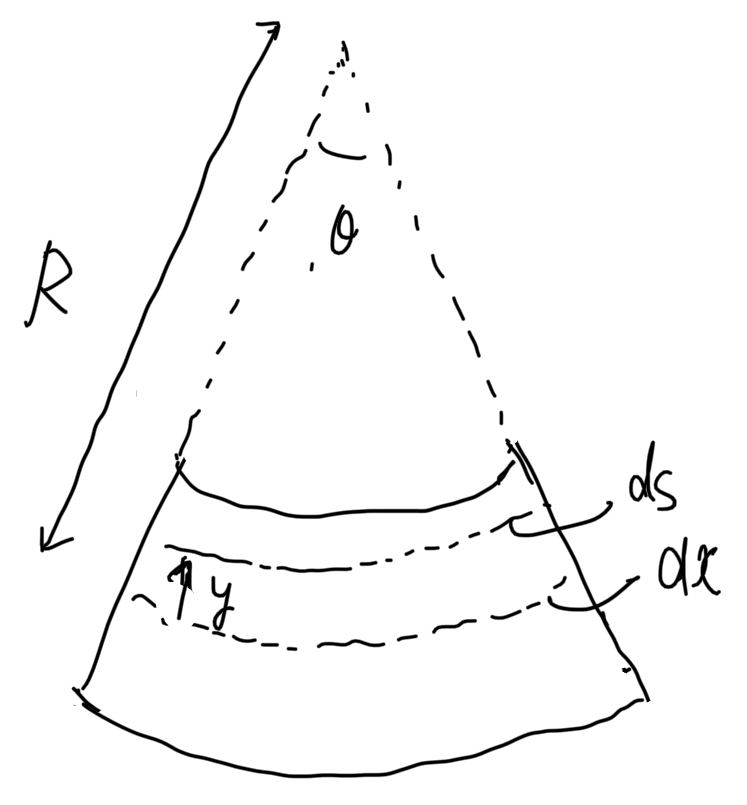
\includegraphics[width=0.3\hsize]{fig1.png}
  \caption{梁の微小部分の変形}
\end{figure}
中立軸から$y$離れた部分の変形後の長さを$ds$とする。
中立軸ではひずみが0であるから、
\begin{align}
  R \theta &= dx \\
  (R - y) \theta &= ds 
\end{align}
が成り立つ。これより、軸ひずみ$\varepsilon$は
\begin{equation}
  \varepsilon = \frac{ds - dx}{dx} = -\frac{y}{R}
\end{equation}
である。

\subsection{}
中立軸が$y = c$にあるとして、式(3)より軸ひずみは
\begin{equation}
  \varepsilon = -\frac{y - c}{R}
\end{equation}
である。軸力が0であるから、満たすべき条件は、
\begin{equation}
  \int_A E \varepsilon \mathrm{d} A = 0
\end{equation}
である。左辺の積分を計算すると、
\begin{equation}
  \frac{2 b c}{R} \int_0^h E \mathrm{d} y = 0
\end{equation}
である。$E(y) \geq 0$を考えて、式(6)が成り立つには
$c = 0$であれば良い。したがって、中立軸は$y = 0$にある。

\subsection{}
\subsubsection{}
\begin{equation}
  M = \int_A E \varepsilon y \mathrm{d} A
\end{equation}
が成り立つから、
\begin{equation}
  M = -\frac{2 b E_0}{R} \int_0^h y^2 (\alpha + \beta f(y)) \mathrm{d} y
\end{equation}
である。

\subsubsection{}
荷重と境界条件が同一であるからcase1とcase2で$M$は等しい。
case2のほうが
$\int_0^h y^2 (\alpha + \beta f(y)) \mathrm{d} y$
が小さいため、$R$が小さい。曲率半径が小さいということにより、
case2のほうが変形が大きい。

\subsubsection{}
幅を
$b^{\prime} = b \left(1 + \frac{3}{5} h^2\right)$
にする。\par
case1では、
\begin{equation}
  M = -\frac{2 b E_0}{R} \int_0^h y^2 (1 + y^2) \mathrm{d} y
  = -\frac{2 b E_0}{R} \left(\frac{h^3}{3} + \frac{h^5}{5}\right)
\end{equation}
である。\par
$E = E_0$のもとで、幅を
$b^{\prime} = b \left(1 + \frac{3}{5} h^2\right)$
とすると、
\begin{equation}
  M = -\frac{2 b^{\prime} E_0}{R} \int_0^h y^2 \mathrm{d} y
  = -\frac{2 b E_0}{R} \left(\frac{h^3}{3} + \frac{h^5}{5}\right)
\end{equation}
である。

\subsubsection{}
断面内で応力は$y = -h$で最大になる。case1では、
\begin{equation}
  \sigma(y = -h) = E(-h) \frac{h}{R}
  = \frac{E_0 (1 + h^2) h}{R}
\end{equation}
である。c)の方法では、
\begin{equation}
  \sigma(y = -h) = E(-h) \frac{h}{R}
  = \frac{E_0 h}{R}
\end{equation}
である。$R$を共通とすると、最大応力は異なる。

\subsection{}
式(8)と
$\frac{1}{R} = \frac{\mathrm{d}^2 w}{\mathrm{d} x^2}$より、
\begin{equation}
  M = -2 b E_0 \frac{\mathrm{d}^2 w}{\mathrm{d} x^2} \int_0^h y^2 (\alpha + \beta f(y)) \mathrm{d} y
\end{equation}
が得られる。
\begin{figure}[htb]
  \centering
  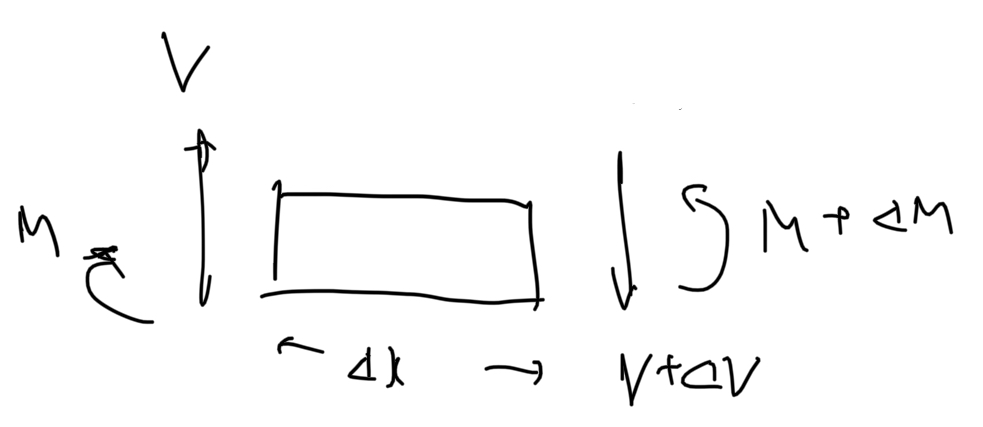
\includegraphics[width=0.3\hsize]{fig2.png}
  \caption{微小部分における断面力}
\end{figure}
ここで、図2のように、長さが$\varDelta x$の微小部分における断面力を考える。
このとき、鉛直方向の力のつり合いとモーメントのつり合いより、
\begin{align}
  V - (V + \varDelta V) &= 0 \\
  M + \varDelta M - M - V \varDelta x &= 0
\end{align}
すなわち、
\begin{align}
  \frac{\varDelta V}{\varDelta x} &= 0 \\
  V &= \frac{\varDelta M}{\varDelta x}
\end{align}
が成り立つ。$\varDelta x \to 0$の極限として、
\begin{align}
  \frac{\mathrm{d} V}{\mathrm{d} x} &= 0 \\
  V &= \frac{\mathrm{d} M}{\mathrm{d} x}
\end{align}
が得られる。よって、
\begin{equation}
  \frac{\mathrm{d}^2 M}{\mathrm{d} x^2} = 0
\end{equation}
が成り立つ。式(13)を式(20)に代入すると、
\begin{equation}
  \frac{\mathrm{d}^4 w}{\mathrm{d} x^4} = 0
\end{equation}
が得られる。

\subsection{}
上側の梁の曲率半径と曲げモーメントをそれぞれ
$R_{up}, M_{up}$とする。下側の梁についても同様に
$R_{low}, M_{low}$を定める。
上側の梁と下側の梁のそれぞれについて、式(7)を計算すると、
\begin{align}
  M_{up} &= \int_0^b \int_{-\frac{h}{2}}^{\frac{h}{2}}
  E_0 \left\{1 + \left(y + \frac{h}{2}\right)^2\right\}
  \left(-\frac{y}{R_{up}}\right) y \mathrm{d} y \mathrm{d} z
  = -\frac{2 b E_0}{R_{up}} \int_0^{\frac{h}{2}}
  \left\{y^4 + \left(\frac{h^2}{4} + 1\right) y^2\right\} \mathrm{d} y \\
  M_{low} &= \int_0^b \int_{-\frac{h}{2}}^{\frac{h}{2}}
  E_0 \left\{1 + \left(y - \frac{h}{2}\right)^2\right\}
  \left(-\frac{y}{R_{low}}\right) y \mathrm{d} y \mathrm{d} z
  = -\frac{2 b E_0}{R_{low}} \int_0^{\frac{h}{2}}
  \left\{y^4 + \left(\frac{h^2}{4} + 1\right) y^2\right\} \mathrm{d} y
\end{align}
となる。上側の梁と下側の梁について荷重と境界条件が同一であるから、
$M_{up} = M_{low}$であり、式(22), (23)より
$R_{up} = R_{low}$となる。
曲率半径が同じであるから、変形の大きさも同じである。

\section{}
\subsection{}
$p_0 = 0$のときのつり合い位置を$x = 0$として、運動方程式は
\begin{equation}
  m \ddot{x} + c \dot{x} + kx = p_0
\end{equation}
である。

\subsection{}
$v = \frac{\omega_0 L}{2 \pi}$を考慮すると、運動方程式は
\begin{equation}
  m \ddot{x} + c \dot{x} + kx =
  \begin{cases}
    P_0 \sin \frac{\omega_0}{2} t & (0 \leq t \leq \frac{L}{v}) \\
    0 & (t < 0, t > \frac{L}{v})
  \end{cases}
\end{equation}
となる。\par
$0 \leq t \leq \frac{L}{v}$のとき、強制振動に対する定常応答は
\begin{equation}
  x_p = \frac{P_0}{k} \frac{1}{1 - \left(\frac{1}{2}\right)^2} \sin \frac{\omega_0}{2} t
  = \frac{4 P_0}{3k} \sin \frac{\omega_0}{2} t
\end{equation}
である。したがって、応答は定数$A,B$を用いて
\begin{equation}
  x = \frac{4 P_0}{3k} \sin \frac{\omega_0}{2} t + A \cos \omega_0 t + B \sin \omega_0 t
\end{equation}
と表せる。初期条件
$x(0) = 0, \dot{x}(0) = 0$を満たすように$A,B$を決定し、
\begin{equation}
  x = \frac{4 P_0}{3k} \sin \frac{\omega_0}{2} t
  - \frac{2 P_0}{3k} \sin \omega_0 t
\end{equation}
を得る。\par
$t > \frac{L}{v}$のとき、応答は定数$C,D$を用いて
\begin{equation}
  x = C \cos \omega_0 \left(t - \frac{L}{v}\right)
  + D \sin \omega_0 \left(t - \frac{L}{v}\right)
\end{equation}
と表せる。式(28)により決まる初期条件
\begin{equation}
  x\left(\frac{L}{v}\right) = 0, \dot{x}\left(\frac{L}{v}\right) = -\frac{4 P_0 \omega_0}{3k}
\end{equation}
を満たすように$C, D$を決定すると、
\begin{equation}
  x = -\frac{4 P_0}{3 k} \sin \omega_0 \left(t - \frac{L}{v}\right)
  = -\frac{4 P_0}{3 k} \sin (\omega_0 t - 2 \pi)
  = -\frac{4 P_0}{3 k} \sin \omega_0 t
\end{equation}
を得る。
したがって、求める応答は、
\begin{equation}
  x =
  \begin{cases}
    \frac{4 P_0}{3k} \sin \frac{\omega_0}{2} t
    - \frac{2 P_0}{3k} \sin \omega_0 t &
    \left(0 \leq t \leq \frac{L}{v}\right) \\
    -\frac{4 P_0}{3 k} \sin \omega_0 t &
    \left(t > \frac{L}{v}\right)
  \end{cases}
\end{equation}
である。

\subsection{}
$p_i(t) = p_0(t - t_i)$とする。これに対する応答を$x_i(t)$とすると、
$p_1(t) = \sum_{i = 0}^n p_i(t)$に対する応答は、
$x(t) = \sum_{i = 0}^n x_i(t)$である。
式(32)の時間をずらすことにより、
\begin{equation}
  x_i(t) =
  \begin{cases}
    0 & (0 \leq t < t_i) \\
    \frac{4 P_0}{3k} \sin \frac{\omega_0}{2} (t - t_i)
    - \frac{2 P_0}{3k} \sin \omega_0 (t - t_i) &
    (t_i \leq t < t_{i+1}) \\
    -\frac{4 P_0}{3 k} \sin \omega_0 (t - t_i) &
    (t_{i+1} \leq t)
  \end{cases}
\end{equation}
である。ここに$t = t_j$を代入すると、
\begin{equation}
  x_i(t_j) =
  \begin{cases}
    0 & (j < i) \\
    \frac{4 P_0}{3k} \sin \frac{\omega_0}{2} (t_j - t_i)
    - \frac{2 P_0}{3k} \sin \omega_0 (t_j - t_i) &
    (j = i) \\
    -\frac{4 P_0}{3 k} \sin \omega_0 (t_j - t_i) &
    (j > i)
  \end{cases}
\end{equation}
$\omega_0 (t_j - t_i) = 2 \pi (j - i)$であるから、
\begin{equation}
  x_i(t_j) = 0 \quad (j = 0, 1, \cdots, n)
\end{equation}
となる。したがって、$j = 0, 1, \cdots ,n$に対して、
\begin{equation}
  x(t_j) = \sum_{i = 0}^n x_i(t_j) = 0
\end{equation}
である。つまり、
\begin{equation}
  x(t_i) = 0 \quad (i = 0, 1, \cdots ,n)
\end{equation}
である。\par
式(33)を微分すると、
\begin{equation}
  \dot{x}_i(t) =
  \begin{cases}
    0 & (0 \leq t < t_i) \\
    \frac{2 P_0 \omega_0}{3k} \cos \frac{\omega_0}{2} (t - t_i)
    - \frac{2 P_0 \omega_0}{3k} \cos \omega_0 (t - t_i) &
    (t_i \leq t < t_{i+1}) \\
    -\frac{4 P_0 \omega_0}{3 k} \cos \omega_0 (t - t_i) &
    (t_{i+1} \leq t)
  \end{cases}
\end{equation}
ここに$t = t_j$を代入すると、
\begin{equation}
  \dot{x}_i(t_j) =
  \begin{cases}
    0 & (j < i + 1) \\
    -\frac{4 P_0 \omega_0}{3 k} & (j \geq i + 1)
  \end{cases}
\end{equation}
であるから、
\begin{equation}
  \dot{x}(t_j) = \sum_{i = 0}^n \dot{x}_i(t_j) =
  \begin{cases}
    0 & (j = 0) \\
    \sum_{i = 0}^{j - 1} \left(-\frac{4 P_0 \omega_0}{3 k}\right)
    & (j \neq 0)
  \end{cases}
  = -\frac{4 j P_0 \omega_0}{3 k}
\end{equation}
となる。したがって、
\begin{equation}
  \dot{x}(t_i) = -\frac{4 i P_0 \omega_0}{3 k} \quad (i = 0, 1, \cdots ,n)
\end{equation}
を得る。

\subsection{}
減衰の性能を高める。車両通過後に生じる自由振動が持続しなくなり、重ね合う振動が減らせる。\par
固有振動数を変える。異なる車両の通過に起因する自由振動が同位相でなくなり強め合わなくなる。
\end{document}